\documentclass[hidelinks, 12pt, a4paper]{article}

\usepackage[margin=0.5in]{geometry}
\usepackage[sfdefault,light]{roboto}
\usepackage[none]{hyphenat}%Remove hyphenation
\usepackage{fontawesome}
\usepackage{hyperref}
\usepackage{tabularx}
\usepackage{tikz}
\usepackage{graphbox}

 \hypersetup{
	colorlinks=true,
	linkcolor=blue,
	filecolor=blue,
	citecolor = black,      
	urlcolor=blue,
}

%No page numbering
\pagenumbering{gobble}
\setlength{\parindent}{0pt}

\begin{document}
	\begin{tabular}{p{0.65\textwidth}p{0.35\textwidth}}
		\begin{minipage}{\linewidth}
			\begin{Huge}Steven Waterman\end{Huge}
			
			\hspace{24pt}\begin{large}Senior Developer at NHS BSA\end{large}\\
			
			I'm a track-proven generalist, able to quickly learn new tech or languages and work across many domains.\\
			
			I can follow best practices, but know how to think outside the box and build reliable solutions when best practice is unrealistic.\\
			
			I'm always happy to spend my time helping others, because in the end it's the users that win --- that's what matters.\\
			
			I'm really ambitious and need to be challenged, flourishing in small teams of brilliant people who will push me to be a better developer.
		\end{minipage} & \vspace{-40pt}\begin{minipage}{\linewidth}
			\begin{flushright}
				\begin{tabular}{rc}
					\href{https://en.wikipedia.org/wiki/Durham,_England}{Durham, UK} & \href{https://en.wikipedia.org/wiki/Durham,_England}{\faHome} \\
					\href{mailto:cv@stevenwaterman.uk}{cv@stevenwaterman.uk} & \href{mailto:cv@stevenwaterman.uk}{\faEnvelope} \\
					\href{http://www.stevenwaterman.uk}{stevenwaterman.uk} & \href{http://www.stevenwaterman.uk}{\faLink} \\
					&\\
					\href{https://www.linkedin.com/in/steven-waterman/}{steven-waterman} & \href{https://www.linkedin.com/in/steven-waterman/}{\faLinkedin} \\
					\href{https://twitter.com/SteWaterman}{SteWaterman} & \href{https://twitter.com/SteWaterman}{\faTwitter} \\
					\href{https://github.com/stevenwaterman}{StevenWaterman} & \href{https://github.com/stevenwaterman}{\faGithub}
				\end{tabular}
			\end{flushright}
		\end{minipage}
	\end{tabular}

	\vspace{12pt}

	\begin{Large}Experience\end{Large}
	\rule{200pt}{1pt}\\
	
	\vspace{-2pt}
	
	\begin{tabularx}{\linewidth}{X r}
		\textbf{Senior Developer @ \href{https://www.nhsbsa.nhs.uk/}{NHS BSA}} & \textbf{Nov 2020 --- Present}
	\end{tabularx}\vspace{2pt}

	\hspace{0.05\linewidth}\begin{minipage}{0.95\linewidth}
		I'm a full stack developer working on the new NHS Jobs, a public-facing Government service.
		Day-to-day, I perform a wide range of work, from fixing accessibility in CSS, improving performance by tweaking SQL, or debugging our containerisation setup.\\
		
		Between tickets, I have a personal focus on developer experience and tooling.
		Shortly after joining, I set up Docker Compose for local development and onboarded the team, meaning nobody is running 15 microservices manually any more.
		I also refactored our frontend integration tests, creating a custom DSL that makes it easier to do things right.\\
		
		I constantly push for more communication between functions, talking to everyone involved and building a high-level understanding of the service to inform future decisions.
		I ran retrospectives with a focus on action, making it more than just a place to vent and giving the team ownership over our ways of working, moving towards a more engaged and collaborative group.\\
	\end{minipage}
	
	
	\begin{tabularx}{\linewidth}{X r}
		\textbf{Developer @ \href{https://www.scottlogic.com/}{Scott Logic}} & \textbf{Aug 2019 --- Oct 2020}
	\end{tabularx}\vspace{2pt}
	
	\hspace{0.05\linewidth}\begin{minipage}{0.95\linewidth}
		As a consultant I worked on a number of demanding projects, often expected to pick up new languages, technologies, or business domains, and be able to contribute within a few days.\\
		
		As the COVID-19 pandemic set in, I worked in a 2/3 person team advising NHS Digital on how to modernise the data pipeline feeding the Shielding Patients List.
		We architected and oversaw the in-place migration from complex SQL queries to a Databricks cluster, ran detailed knowledge transfer sessions, and advised senior leadership on best practices for Data and DevOps.\\
		
		Prior to that, I was a full-stack web developer on an upcoming product for a multinational bank.
		That project saw me architect and create the inter-service authentication and data auditing functionality, plus guiding the team on type-safe and scalable frontend development.\\
		
		I also have experience with modern cloud deployment and DevOps practices from my time working on a Twitter-like equities research platform.
		There, I set up continuous deployment with AWS CDK (infrastructure-as-code), including data storage bridging both SQL and NoSQL.\\
	\end{minipage}


	\begin{tabularx}{\linewidth}{X r}
		\textbf{Junior Software Engineer @ \href{https://www.condecoconnect.com/}{Codeco}} & \textbf{Jul 2018 --- Oct 2018}
	\end{tabularx}\vspace{2pt}

	\hspace{0.05\linewidth}\begin{minipage}{0.95\linewidth}
		As an intern working on the backend API, the microservice architecture used at Condeco was completely new to me.
		I spent a few months learning and getting up to speed, culminating in me conceiving, architecting, and pitching a new licencing microservice to technical leadership.
	\end{minipage}
	
	\begin{Large}Education\end{Large}
	\rule{200pt}{1pt}\\
	
	
	\begin{tabularx}{\linewidth}{X r}
		\textbf{\href{https://www.dur.ac.uk/courses/info/?id=11509\&title=Computer+Science\&code=G400\&type=BSC\&year=2016}{BSc Computer Science} @ Durham University (1st Class Hons.)} & \textbf{2016 --- 2019}
	\end{tabularx}\vspace{2pt}

	\hspace{0.05\linewidth}\begin{minipage}{0.95\linewidth}
		Dissertation title: \emph{Tailoring horror games with biosignals}\\
	\end{minipage}

	
	\begin{tabularx}{\linewidth}{X r}
		\textbf{\href{https://www.dur.ac.uk/courses/info/?id=11558\&title=General+Engineering\&code=H100\&type=MENG\&year=2015}{MEng General Engineering} @ Durham University} & \textbf{2015 --- 2016}
	\end{tabularx}\vspace{2pt}

	\hspace{0.05\linewidth}\begin{minipage}{0.95\linewidth}
		I always wanted to work in tech, but an elective CS module convinced me to change course\\
	\end{minipage}

	
	\vspace{8pt}
	\begin{Large}Other Work\end{Large}
	\rule{200pt}{1pt}\\
	
	
	\begin{tabularx}{\linewidth}{X r}
		\textbf{Thought Leadership} & \textbf{Constantly!}
	\end{tabularx}\vspace{2pt}
	
	\hspace{0.05\linewidth}\begin{tabularx}{0.95\linewidth}{Xr}
		\begin{minipage}{\linewidth}
			I'm a seasoned speaker at local tech talks, including that time I threw chocolates at \href{https://www.youtube.com/watch?v=2ibiA5TEsxw}{NE:Tech} and the time I live-coded an underwhelming website with \href{https://svelte.dev}{Svelte} at \href{https://www.youtube.com/watch?v=P6u0Uv_VxCU}{NE-RPC}.
			I've written many \href{https://stevenwaterman.uk/}{blogs}, including my descent into \href{https://blog.scottlogic.com/2020/10/09/ergo-rabbit-hole.html}{ergo-keyboard madness} that went viral and ended up on the \href{https://news.ycombinator.com/item?id=24728224}{HN front page}.
			I've also made regular appearances in \href{https://www.baeldung.com/java-weekly-315}{Java Weekly} with technical blogs like \href{https://blog.scottlogic.com/2020/01/03/rethinking-the-java-dto.html}{Rethinking the Java DTO}.
		\end{minipage} & \href{https://blog.scottlogic.com/2020/10/09/ergo-rabbit-hole.html}{
\includegraphics[align=c, width=0.36\textwidth]{keyboard}}
	\end{tabularx}

	\vspace{24pt}
	
	\begin{tabularx}{\linewidth}{X r}
		\textbf{Narration.studio} (\href{https://narration.studio/}{Live}) (\href{https://github.com/stevenwaterman/narration.studio/}{GitHub}) & \textbf{Oct 2020}
	\end{tabularx}\vspace{2pt}

	\hspace{0.05\linewidth}\begin{tabularx}{0.95\linewidth}{Xr}
		\begin{minipage}{\linewidth}
			When I narrated my ergo-keyboard blog post, it was a really tedious manual process.
			That was no good, so I made Narration.studio: an in-browser narration editing tool using the web speech recognition API to be completely hands-free.
			Read the lines of your script as they appear on screen, and redo a line by simply saying it again.
			Narration.studio will detect it and overwrite the previous recording for that line.
			Highlighted in the Dec 2020 \href{https://svelte.dev/blog/whats-new-in-svelte-december-2020}{Svelte Community Showcase}.
		\end{minipage} & \href{https://narration.studio/}{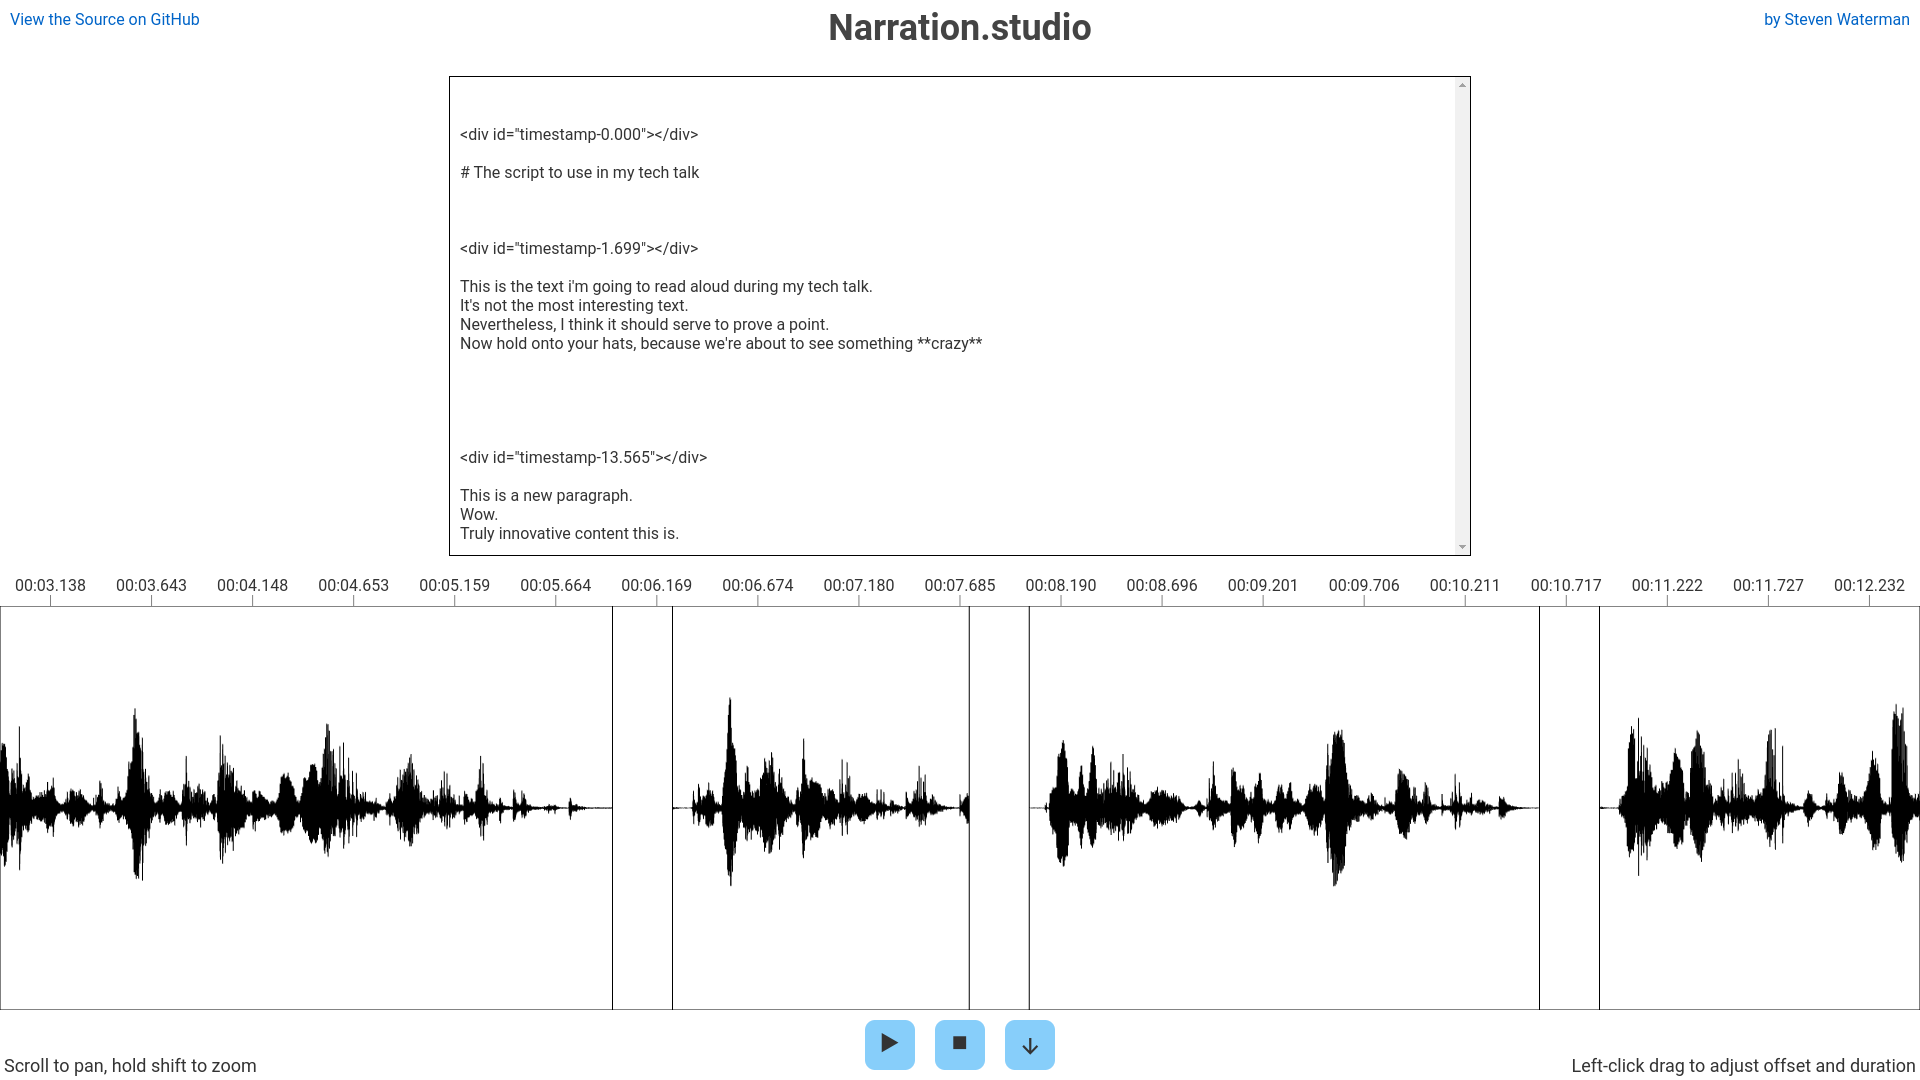
\includegraphics[align=c, width=0.36\textwidth]{narrationstudio}}
	\end{tabularx}
	
	\vspace{24pt}
	
	\begin{tabularx}{\linewidth}{X r}
		\textbf{MuseTree} (\href{https://stevenwaterman.uk/musetree/}{Live}) (\href{https://github.com/stevenwaterman/musetree}{GitHub}) & \textbf{Jan 2020}
	\end{tabularx}\vspace{2pt}
	
	\hspace{0.05\linewidth}\begin{tabularx}{0.95\linewidth}{Xr}
		\begin{minipage}{\linewidth}
			After falling in love with \href{https://openai.com/blog/musenet/}{MuseNet}, OpenAI's MIDI generator, I decided to make a custom front-end for it.
			While the official tool is a simple toy demo, MuseTree is used by creators in real-world scenarios to create songs and jingles.
			As a successful open-source project, it sees frequent contributions from the FOSS community.
			Latest update adds integration with the Web Audio API to perform real-time audio synthesis in-browser.
		\end{minipage} & \href{https://stevenwaterman.uk/musetree/}{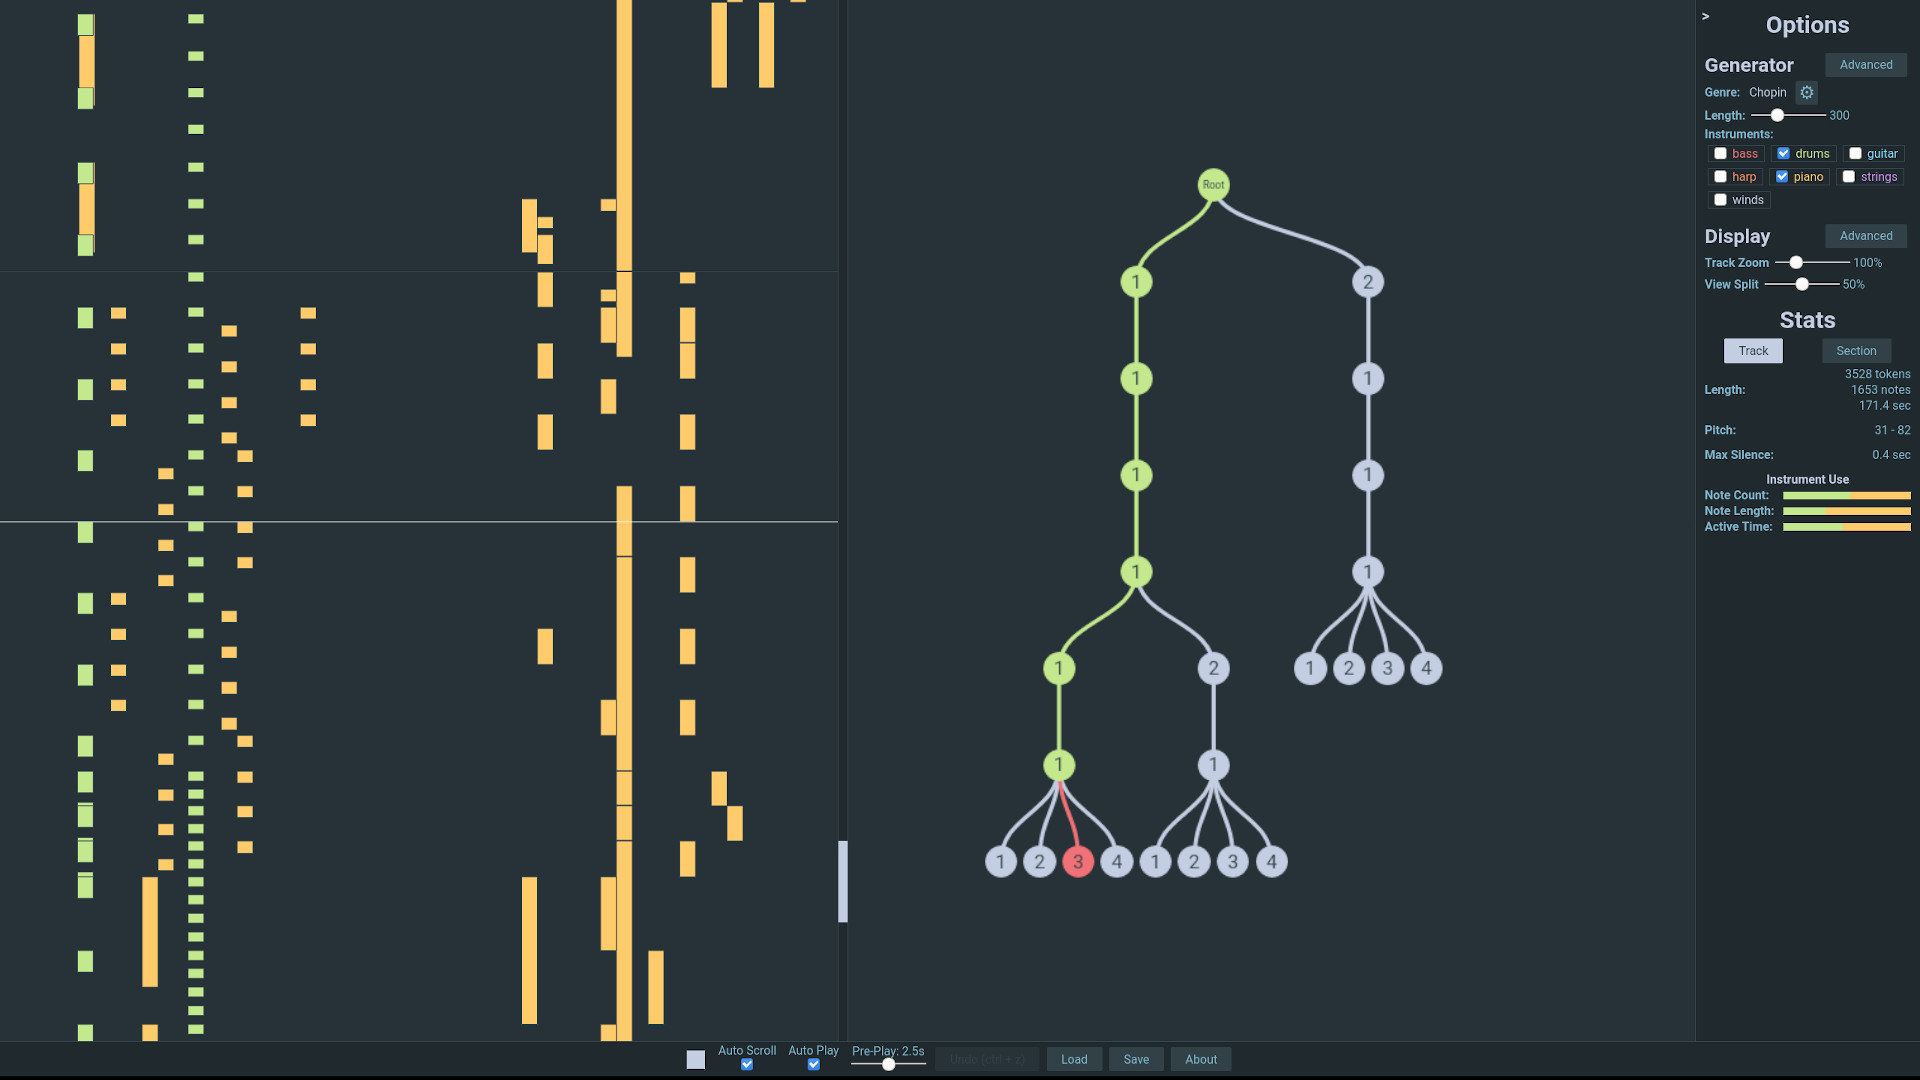
\includegraphics[align=c, width=0.36\textwidth]{musetree}}
	\end{tabularx}

	\vspace{24pt}
	
	\begin{tabularx}{\linewidth}{X r}
		\textbf{Sharpshot} (\href{https://github.com/stevenwaterman/sharpshot}{GitHub}) & \textbf{Dec 2018}
	\end{tabularx}\vspace{2pt}
	
	\hspace{0.05\linewidth}\begin{tabularx}{0.95\linewidth}{Xr}
		\begin{minipage}{\linewidth}
				I created the initial version of Sharpshot in 24 hours for \href{http://www.durhack.com}{Durhack 2018}, winning the `GitHub Prize for Best Dev Tool' \& overall runner-up. It's an esoteric visual programming language where nodes are placed on a grid. Each node represents a function, and parameters move around the screen annihilating each other when they collide. An addictive Zachlike puzzle game.
		\end{minipage} & \href{https://github.com/stevenwaterman/sharpshot}{\includegraphics[align=c, width=0.36\textwidth]{sharpshot}}
	\end{tabularx}
\end{document}